% !TEX root = ./multilinear.tex
\section{Proposed parallel algorithm}
\label{sec:proposed}
We propose a distributed implementation of Algorithm \ref{alg:maxwt} for the $k$-MLD problem. The computation in the recursive step has a \emph{local} structure: a vertex only needs data from its immediate neighbors in the graph. Thus, Algorithm \ref{alg:maxwt} is amenable to a vertex-centric parallelization. However, as we describe below, there are various techniques and implementation details needed to make the computation scalable and overcome high communication overheads. \comment{Someone revise the last 2 sentences, please.} 

%Both problems \ref{prob:trees} and \ref{prob:macs} can be reduced to instances of the $k$-MLD problem, as we will discuss later in Section \ref{sec:applications}; this will automatically lead to corresponding parallel algorithms for both these problems.

\subsection{Overview of the Algorithm \parmaxwt{}}
Let $N$ denote the total number of
processors or parallel units available. Quantities $N_1$ and $N_2$ are parameters for controlling the parallelism
in different parts of the algorithm.  
We assume $2^k/N_2$ and $N/N_1$ are integers, in order to avoid cluttering the
notation using ceiling and floor of these quantities, respectively.
%The algorithm involves solving a dynamic program repeatedly for a certain number of rounds. 
The algorithm involves solving a dynamic program $2^k$ times; these $2^k$ loops are independent, and we divide them into \emph{phases} of size $N_2$ each, so that a total of $2^k/N_2$ phases have to be run. These are run in $2^k/(N_2N/N_1)$ ``batches", where each batch involves running $N/N_1$ phases. A phase involves a call to the subroutine \parcircuit{}.
See Figure \ref{fig:parallel} for an illustration of this structure.

We partition the graph $G$ into $N_1$ parts, denoted by
$\mathcal{P}=\{G^1, \ldots, G^{N_1}\}$; desirable properties of the partition will be discussed later. For a partition $j$, let $\textsc{Deg}(j)$ be the \emph{degree} of $j$, defined as the number of edges connecting nodes in $j$ to nodes in some other partition:
$$
\textsc{Deg}(j) = |\{(u, v): (u, v) \in G, u \in G^i, v \not \in G^i\}|,
$$
and let \maxdeg{} $ = \max_{j} \textsc{Deg}(j)$. Also, let $\maxload{} = \max_j |G^j|$ be the maximum ``load" or number of vertices on any partition. We will analyze the performance of our algorithm in terms of $\maxload{}$ and $\maxdeg{}$.

%\begin{figure}[h]
%\centering
%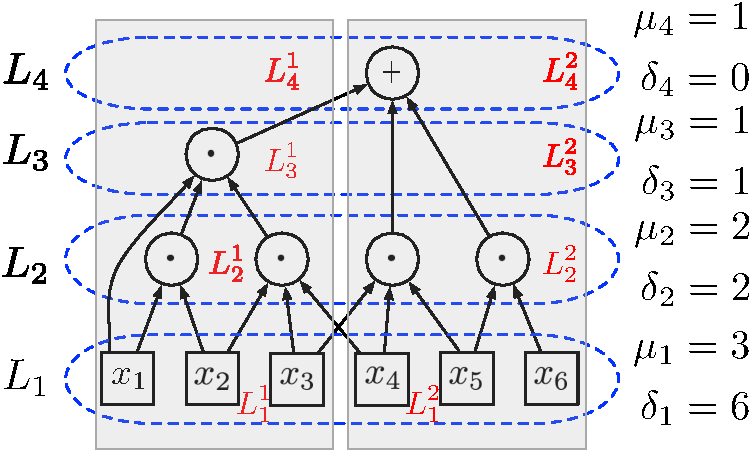
\includegraphics[width=0.4\textwidth]{img/dag4.pdf}
%\caption{
%\small
%Illustration of the level sets and associated quantities for the DAG in
%Figure \ref{fig:dag}, corresponding to a partition into two parts. 
%%\vspace{-0.2in}
%}
%\label{fig:dag4}
%\end{figure}

%\noindent
%\textbf{High level overview.}
We describe the main intuition of the steps of Algorithm \parmaxwt{} below.
\begin{enumerate}
\item
The algorithm starts with the partitioning $\mathcal{P}$ of the graph $G$.
%We discuss its complexity and implementation in Section \ref{sec:partition}.
\item
The algorithm runs $\log{1/\epsilon}\log{5/4}$ rounds, each of which involves $2^k$ iterations.
Here, $\epsilon\in(0, 1)$ is a parameter, which governs the success probability\footnote{As per Theorem \ref{theorem:kmld}, Algorithm \maxwt{} succeeds with probability 1/5, so we need to run it multiple times}. Each such round with $2^k$ iterations is partitioned into
$2^k/N_2$ phases in the while loop in lines 8--12 of \parmaxwt{}, which are completely independent of other phases.
\item
In the $t$th phase, Algorithm \parcircuit{} uses a vector of size $N_2$ to store
$\langle P(i, tN_2),\ldots, P(i, (t+1)N_2-1)\rangle$ for each node $i$; these
will be computed simultaneously using a dynamic program.
\item
In the $t$th phase, for each node $i$, we use the vector for each neighbor $u$ of $i$ to compute $\langle P(i, tN_2),\ldots, P(i, (t+1)N_2-1)\rangle$.
If $u$ is in the same partition, then its data is available on that processor. For every neighbor $u$ in a different partition, $u$ has to send a message with $\langle P(u, tN_2),\ldots, P(u, (t+1)N_2-1)\rangle$, introducing a communication overhead.
\item
We use $\rootsum^{\ell}_t = P(tN_2, k) + \ldots P((t+1)N_2-1, k)$ 
to denote the sum of the values of the root node within the phase, for round $\ell$. These are summed up
over all the phases within round $\ell$ to compute the total, denoted by $P^{\ell}$.
\end{enumerate}

\begin{figure}[h]
\centering
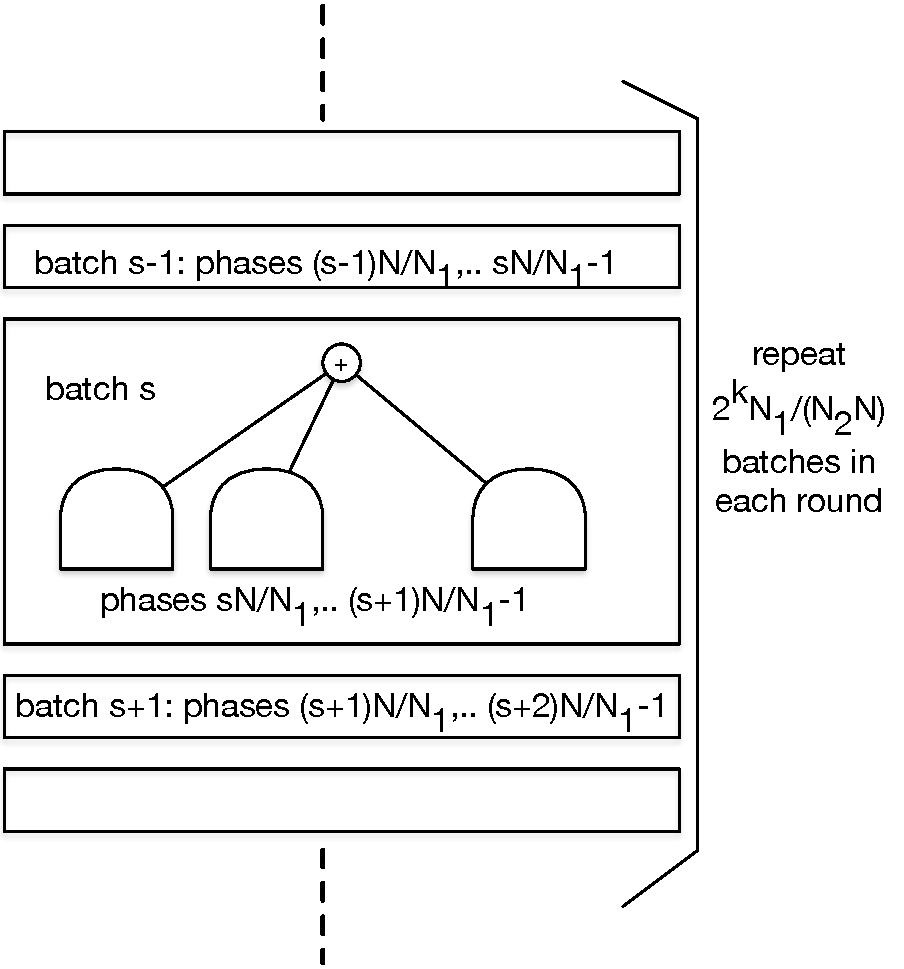
\includegraphics[width=0.3\textwidth]{img/parallel.pdf}
\caption{
\small
Schematic structure of \parmaxwt{}: we run $(\log{1/\epsilon})/(\log{5/4})$ rounds.
Each round is partitioned into $2^kN_1/(N_2N)$ batches, and each batch involves
$N/N_1$ phases being run simultaneously. Each phase involves an evaluation of the
polynomial on $N_2$ iterations in algorithm \parcircuit{}, which are then summed up.
}
\label{fig:parallel}
\end{figure}

\begin{algorithm}{}
\small
\caption{\parmaxwt{}$(G, k, \epsilon, N_1, N_2)$.}
\label{alg:parallel-kMLD} 
\begin{algorithmic}[1]
\STATE \textbf{Input}: Graph $G=(V,E)$, parameter $k$,
confidence parameter $\epsilon\in (0, 1)$, parameters $N_1$ and $N_2$, which guide the parallelism.
\STATE\textbf{Output}: ``Yes" if circuit evaluation is non-zero. ``No" otherwise.

\STATE Let $v_i \in \mathbb{Z}_2^k$ be a random vector for each node $i$
\STATE Let $P = \bar 0$ be the polynomial
\STATE Let $N_1$ denote the number of processors used for each iteration.
%Let $\mathcal{P}=\{G^1= (V^1, E^1), \ldots, G^{N_1}=(V^{N_1}, E^{N_1})\}$ denote the corresponding
Let $\mathcal{P}=\{G^1, \ldots, G^{N_1}\}$ denote the corresponding partition of the graph into $N_1$ parts.
\STATE \textbf{for} $\ell=1$ to $(\log{1/\epsilon})/(\log{5/4})$ 
\STATE \quad $P^{\ell}=0$
\STATE \quad \textbf{while} $s \leq \frac{2^k/N_2}{N/N_1}$ \textbf{do}
\STATE \quad \quad \textbf{for} $t =s N/N_1$ to $(s+ 1)N/N_1$ \textbf{do in parallel}
\STATE \quad \qquad  $\rootsum^{\ell}_{t} = \parcircuit(G, k, \mathbf{v}, t, N_2, N_1, \mathcal{P})$
\STATE \quad \quad \textsc{MpiBarrier}
\STATE \quad \quad $P^{\ell} = P^{\ell} + \sum_{t=s N/N_1}^{(s+1)N/N_1} \rootsum^{\ell}_{t} \mod 2^{k+1}$ using \textsc{MpiReduce}
\STATE \textbf{if} $P^{\ell}\neq 0$ for some $\ell$
\STATE \quad \textbf{return} \textbf{True}
\STATE \textbf{else} 
\STATE \quad \textbf{return} \textbf{False}
\end{algorithmic}
\end{algorithm}

\begin{algorithm}{}
\small
\caption{\parcircuit{$(G, k, \mathbf{v}, t, N_2, N_1, \mathcal{P})$}}
\label{alg:parEvaluate} 
\begin{algorithmic}[1]
%\STATE \textbf{Procedure} \parcircuit{$(G(V, E), k, \mathcal{L}, \mathbf{v}, t, p)$}
\STATE \textbf{Input:} Circuit $G$, parameter $k$, random assignment $\mathbf{v}$, phase number $t$, number of iterations within phase $N_2$, number of partitions $N_1$, and partitioning $\mathcal{P}$
\STATE
\STATE \textbf{for} processor $s$ \textbf{do in parallel}
\STATE \quad \textbf{Base case}
\STATE \quad \textbf{for} node $i \in G^s$ and iteration $q \in tN_2,\ldots,(t+1)N_2-1$ \textbf{do}
\STATE \qquad $ P(i, q, 1) = 1 + (-1)^{v_i^T \cdot q_{\text{bin}}}$

\STATE \quad \textbf{Recursive step}
\STATE \quad \textbf{for} $j=2$ to $k$ \textbf{do}
\STATE \qquad \textbf{for} vertex $i \in G^s$ \textbf{do}
\STATE \qquad \quad \textbf{for} all $q$ set $P(i,q,  j) = \bar 0$
\STATE \qquad \quad \textbf{for} each incoming message $\langle u, P(u, q, [1, j-1])\rangle$ \textbf{do}
\STATE \qquad \qquad $P(i, q, j)=$ $P(i, q, [1, j-1])  P(u, q, [1, j-1])$
\STATE \qquad \quad  \textbf{Send result to neighbors}
\STATE \qquad \quad \textbf{for} $u \in \nbr(i)\setminus G^s$ \textbf{do}
\STATE \qquad \qquad \textbf{Send} $\langle i, P(i, q, j)\rangle$
\STATE \textsc{MpiBarrier}
\STATE \textbf{return} $\sum_q \sum_i P(i, q, k)$
\end{algorithmic}
\end{algorithm}

Recall the definition of $\maxdeg{}$ corresponding to the partitioning $\mathcal{P}$.
Further, let $c_1$ and $c_2$ denote the time for unit computation at any node in $G$
and the unit communication along any edge, respectively, in the Algorithm \parcircuit{}.
The time and communication complexity of algorithm \parmaxwt{} is summarized below
in terms of these parameters. 

\begin{theorem}
\label{thm:parmaxwt}
For any $\epsilon\in(0, 1)$,
Algorithm \parmaxwt{} solves the \textsc{$k$-MLD} problem for an
instance $P(x_1,\ldots,x_n)$ with probability at least $1-\epsilon$. The total time for
computation and communication are $O\left(c_1\frac{2^kN_1}{N}k \maxload{}\log{1/\epsilon}\right)$ 
and $O\left(c_2\frac{2^kN_1}{N N_2}k \maxdeg{}\log{1/\epsilon}\right)$, respectively.
\end{theorem}
\begin{proof} (Sketch)
First, we argue the correctness. 
The call to \parcircuit{} evaluates the polynomial bottom up in parallel for all iterations in the
$t$th phase, namely iterations $tN_2,\ldots,(t+1)N_2-1$. The vector
$\langle P(tN_2, k),  \ldots ,P((t+1)N_2-1, k)\rangle$
is the final evaluation of the polynomial for each iteration in this phase.
Each call to \parcircuit{} in Algorithm \parmaxwt{}
returns the sum of these values for phase $t$.
Each round of Algorithm \parmaxwt{}, corresponding to the value of
$\ell$ in the outer for loop in lines 6--12, goes over all phases, and
calls \parcircuit{}. Therefore, within round $\ell$, $P^{\ell}$ denotes the
sum of the polynomial evaluation over all the $2^k$ iterations within that round.
If $P(\cdot)$ has a multilinear term,
from \cite{koutis:icalp08,williams2009finding}, $P^{\ell}\neq 0 \text{ mod }2^{k+1}$ with
probability at least $1/5$. This implies that 
$\Pr[P^{\ell} = 0,\ \forall \ell] = (\frac{4}{5})^{(\log{1/\epsilon})/(\log{5/4})}\leq\epsilon$,
so that with probability at least $1-\epsilon$, \parmaxwt{} returns true.  On the other hand,
if $P(\cdot)$ has no multilinear term, then with probability $1$, $P^{\ell}=0$ for all $\ell$.
Therefore, \parmaxwt{} correctly solves the \textsc{$k$-MLD} problem with probability
at least $1-\epsilon$.

Next, we consider the computation and communication time complexity. 
The algorithm \parcircuit{} computes the polynomial for each degree up to $k$ within each iteration.
Therefore, the computation time in a phase $t$ is 
$O(c_1 k \max_j |G^j| N_2) = O(c_1k\maxload{}N_2)$, which is the maximum time for any processor. Therefore, the total compute time over all the rounds is
$O(\frac{2^k/N_2}{N/N_1} c_1 k \maxload{} N_2)$, which corresponds to the bound in the theorem.
After any evaluation in the recursive step, the results have to be sent on all neighbors, for every pair of
processors $s, s'$. Therefore, the maximum number of messages in one iteration of the loop in lines 8--15 is $\maxdeg{}$, and the total number of messages, over all the rounds, is
$O(\frac{2^k/N_2}{N/N_1} \maxdeg{}) = O(\frac{2^kN_1}{N N_2} \maxdeg{})$.
\end{proof}

%%\subsection{Partition and Load Balancing}
%%\label{sec:partition}
%%
%%From Theorem \ref{thm:parmaxwt}, the performance of Algorithm \parmaxwt{} depends crucially
%%on the partitioning. Specifically, the partition should be ``vertical'', i.e., one which achieves
%%load balance across each level and also minimizes the edge cut, which is formalized by
%%\[
%%\text{cost}(\mathcal{P}) = \sum_s (c_1\maxload{}_s + c_2\maxdeg{}_s)
%%\]
%%
%%However, finding a partitioning $\mathcal{P}$ that minimizes the above objective
%%$\text{cost}(\mathcal{P})$ is NP-hard, in general, as summarized below. The proof
%%is omitted for brevity.
%%
%%\begin{lemma}
%%\label{lemma:partition}
%%Given a DAG $G=(V, E)$ and per-unit computation and communication costs $c_1$ and $c_2$,
%%respectively, finding a partitioning $\mathcal{P}$ with the minimum cost is NP-hard, in general.
%%\end{lemma}
%%
%%In light of Lemma \ref{lemma:partition}, we consider two heuristics: finding balanced
%%partitions in each level, and combining them, as well as METIS \cite{karypis:sijsc99}.

%We partition the circuit ``vertically"; that is, each processor gets a subset of nodes for each level in $\mathcal{L}$. Let $f(i)$ be the cost of evaluating node $v$. Then, we want to find a partition, such that
%$$
%\sum_{v \in V^p} f(i) \approx \frac{1}{p}\sum_{i \in V} f(i).
%$$

%\subsection{Analysis of Algorithm \parmaxwt{}}
%\subsubsection{Time Complexity}
%The \textbf{while} loop in lines 8--13 of \parmaxwt{} runs for at most $\frac{2^k}{P / p}$ iterations. For each iteration, each partition does work in the order $O(\frac{1}{p}\sum_{i \in V} f(i))$, so the total running time is $O(\frac{1}{p}(2^k f(V)))$.
%\subsubsection{Number of Messages}
%We assume that we have $P$ processors available and that $G$ does not fit in the memory of a single computing node. We have to use $p \leq P$ processors to store the graph in memory. We propose an MPI algorithm with roughly the following steps:

%\begin{enumerate}
%\item \parmaxwt{} Algorithm \ref{alg:parallel-kMLD}
%\item Determine $p$, the number of processors needed to store the graph.
%\item We have to run the loop from line 9 of \maxwt{}. Each of the $2^k$ iteration is independent of the others, so we can run $\lfloor{P/p}\rfloor$ iterations in parallel.
%\item \parcircuit{} Algorithm \ref{alg:parEvaluate}
%\item For each iteration $t$, we first partition the circuit into $p$ parts, and we evaluate these parts in parallel.
%\item For each partition $p'$, we evaluate the circuit by levels, as in \maxwt{}. 
%\item For each node $i$ that we evaluate, we compute $m(i)$ using the $m(j)$ value for each predecessor $j$. if a predecessor $j$ is in the same partition $p'$, then, we can simply read $m(j)$, as in the sequential algorithm. For every predecessor $j$ in a different partition, $j$ has to send a message with $m(j)$, introducing a communication overhead.
%\item We aggregate the value at root$(G)$ over all $2^{k}$ iterations to get the final solution.
%\end{enumerate}

%\noindent
%\textbf{Algorithm \ref{alg:parallel-kMLD}}: \parmaxwt{}\\
%1. Determine $p$, the number of processors needed to store the graph.\\
%2. We have to run the loop from line 9 of \maxwt{}. Each of the $2^k$ iteration is independent of the others, so we can run $\lfloor{P/p}\rfloor$ iterations in parallel.\\
%\textbf{Algorithm \ref{alg:parEvaluate}}: \parcircuit{} \\
%3. For each iteration $t$, we first partition the circuit into $p$ parts, and we evaluate these parts in parallel.\\
%4. For each partition $p'$, we evaluate the circuit by levels, as in \maxwt{}. \\
%5. For each node $i$ that we evaluate, we compute $m(i)$ using the $m(j)$ value for each predecessor $j$. If a predecessor $j$ is in the same partition $p'$, then, we can simply read $m(j)$, as in the sequential algorithm. For every predecessor $j$ in a different partition, $j$ has to send a message with $m(j)$, introducing a communication overhead.\\
%6. We aggregate the value at root$(G)$ over all $2^{k}$ iterations to get the final solution.
